\documentclass [12pt]{article}
\usepackage{tikz,pgfplots}
\usetikzlibrary{arrows,calc}
\newenvironment{customlegend}[1][]{%
    \begingroup
    % inits/clears the lists (which might be populated from previous
    % axes):
    \csname pgfplots@init@cleared@structures\endcsname
    \pgfplotsset{#1}%
}{%
    % draws the legend:
    \csname pgfplots@createlegend\endcsname
    \endgroup
}%

% makes \addlegendimage available (typically only available within an
% axis environment):
\def\addlegendimage{\csname pgfplots@addlegendimage\endcsname}

%%--------------------------------

% definition to insert numbers
\pgfkeys{/pgfplots/number in legend/.style={%
        /pgfplots/legend image code/.code={%
            \node at (0.295,-0.0225){#1};
        },%
    },
}
%%===================================

\begin{document}

\begin{center}
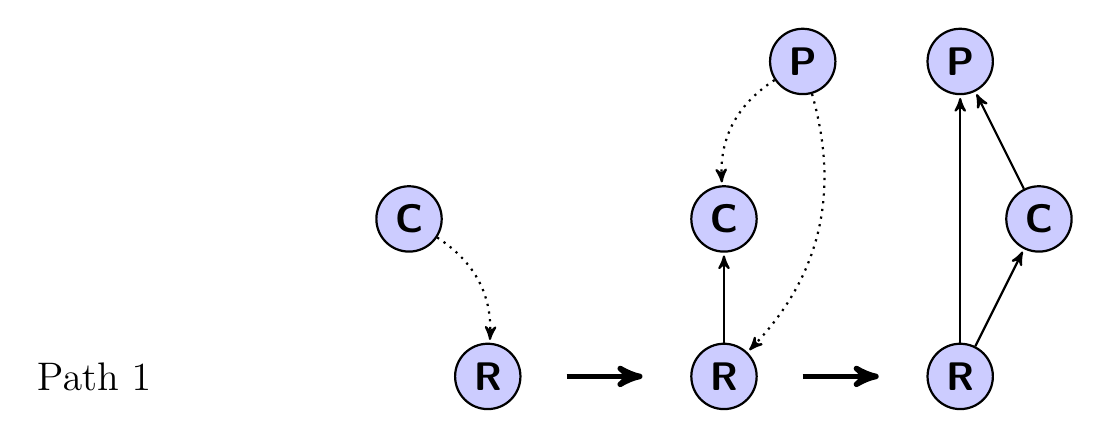
\begin{tikzpicture}[->,>=stealth',shorten >=1pt,auto,
  thick,main node/.style={circle,fill=blue!20,draw,font=\sffamily\Large\bfseries}]

\node[main node](R1) at (1,0) { R};
\node[main node](C1) at (0,2) {C};
\node[main node](C2) at  (4,2){C};
\node[main node](R2) at ($(R1) + (3,0)$) {R};
\node[main node](P1) at (5,4){P};
\node[main node](R3) at ($(R2) + (3,0)$){R};
\node[main node](C3) at ($(R3) + (1,2)$){C};
\node[main node](P3) at ($(R3) + (0,4)$){P};
\node[font = \fontsize{15}{15}\selectfont](A1) at (-4,0) {Path 1};

\path
(C1) edge[bend left,dotted] (R1)
($(R1)+(1.0,0)$) edge[line width = 2]  ($(R1)+ (2,0)$)
(R2) edge (C2)
(P1) edge[bend right,dotted] (C2)
(P1) edge[bend left,dotted] (R2)
($(R2) + (1.0,0)$) edge[line width  = 2] ($(R2) + (2,0)$)
(R3) edge (C3)
(R3) edge (P3)
(C3) edge (P3);
\end{tikzpicture}
$\left. \right.$\\
$\left. \right.$\\

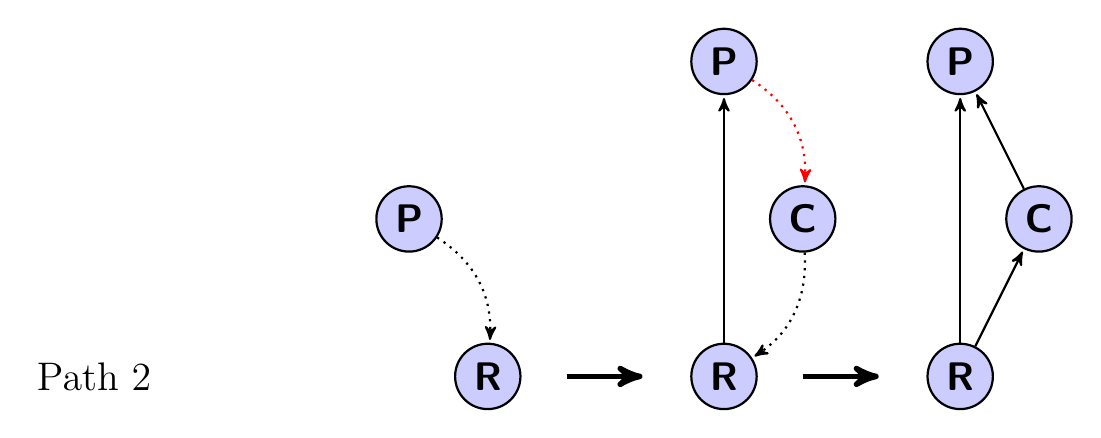
\begin{tikzpicture}[->,>=stealth',shorten >=1pt,auto,
  thick,main node/.style={circle,fill=blue!20,draw,font=\sffamily\Large\bfseries}]

\node[main node](R1) at (1,0) { R};
\node[main node](P1) at (0,2) {P};
\node[main node](P2) at  (4,4){P};
\node[main node](R2) at ($(R1) + (3,0)$) {R};
\node[main node](C1) at (5,2){C};
\node[main node](R3) at ($(R2) + (3,0)$){R};
\node[main node](C3) at ($(R3) + (1,2)$){C};
\node[main node](P3) at ($(R3) + (0,4)$){P};
\node[font = \fontsize{15}{15}\selectfont](A1) at (-4,0) {Path 2};

\path
(P1) edge[bend left,dotted] (R1)
($(R1)+(1.0,0)$) edge[line width = 2]  ($(R1)+ (2,0)$)
(R2) edge (P2)
(C1) edge[bend left,dotted] (R2)
(P2) edge[bend left,dotted,red] (C1)
($(R2) + (1.0,0)$) edge[line width  = 2] ($(R2) + (2,0)$)
(R3) edge (C3)
(R3) edge (P3)
(C3) edge (P3);

\end{tikzpicture}
\end{center}
\end{document}